\documentclass[letter,11pt]{article}

\usepackage[spanish,es-nodecimaldot]{babel}
\usepackage[utf8]{inputenc}

\usepackage{lmodern}
\usepackage[T1]{fontenc}
\usepackage{textcomp}

\usepackage{framed}
\usepackage[svgnames]{xcolor}
\colorlet{shadecolor}{Gainsboro!50}

\usepackage{enumitem}
\usepackage{graphicx}
\usepackage{pstricks}

\usepackage{anysize}
\marginsize{3cm}{2cm}{2cm}{3cm}

\usepackage{siunitx}
\usepackage{amsmath}
\usepackage{array}
\usepackage{alltt}

\usepackage{fancyhdr}
\usepackage{lastpage}
\pagestyle{fancy}
\fancyhf{}
\fancyhead[LE,RO]{Física Básica II}
\fancyfoot[CO,CE]{\thepage\ de \pageref{LastPage}}

\special{papersize=215.9mm,279.4mm}

\usepackage[
    pdfauthor={Carlos Eduardo Caballero Burgoa},%
    pdftitle={Física Básica II},%
    pdfsubject={Tarea 5},%
    colorlinks,%
    citecolor=black,%
    filecolor=black,%
    linkcolor=black,%
    urlcolor=black,
    breaklinks]{hyperref}
\usepackage{breakurl}

\newcommand{\blankpage}{
\newpage
\thispagestyle{empty}
\mbox{}
\newpage
}

\renewcommand{\arraystretch}{1.2}

\begin{document}

\begin{center}
    {\Large \bf{\underline{Tarea \#5}}}
\end{center}

Determinar el centro de masa de una barra delgada inclinada $30\si{\degree}$ con
respecto a la horizontal. La masa de la barra es $M$ y su longitud es $L$.

\begin{figure}[!h]
\centering
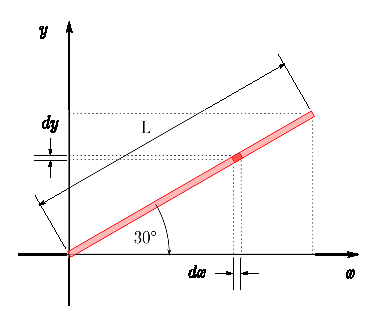
\includegraphics[scale=1.20]{resources/f1.eps}
\end{figure}

\vspace{1.0cm}
\textbf{\underline{Solución}:} \\

Dada la ecuación del centro de masa:

\begin{equation}
    \vec{r}_{cm} = \frac{1}{M} \int_{M} \vec{r} \cdot dm
\label{base}
\end{equation}

Asumiendo la distribución homogénea de la masa sobre el material:
\begin{equation*}
    \lambda = \frac{dm}{dl} = ctte
\end{equation*}

Por tanto:
\begin{equation}
    dm = \lambda \cdot dl
\label{dm}
\end{equation}

Reemplazando (\ref{dm}) en (\ref{base}):
\begin{equation*}
    \vec{r}_{cm} = \frac{1}{M} \int_{0}^{L} \vec{r} \cdot \lambda \cdot dl
\end{equation*}

Reemplazando $\vec{r}$ por sus componentes:
\begin{equation*}
    \vec{r}_{cm} = \frac{1}{M} \int_{0}^{L} (x \hat{i} + y \hat{j}) \cdot \lambda \cdot dl
\end{equation*}

Realizando los siguientes cambios de variable:
\begin{equation}
    dx = dl \cdot cos(30\si{\degree})
\label{dx}
\end{equation}
\begin{equation}
    dy = dl \cdot sen(30\si{\degree})
\label{dy}
\end{equation}

Para $\hat{i}$ obtenemos:
\begin{equation*}
    x_{cm} = \frac{1}{M} \int_{0}^{L} x \cdot \lambda \cdot dl = \frac{1}{M} \int \frac{x \cdot \lambda \cdot dx}{cos(30\si{\degree})} = \frac{\lambda}{M \cdot cos(30\si{\degree})} \int_{0}^{L \cdot cos(30\si{\degree})} x \cdot dx
\end{equation*}
\begin{equation*}
    x_{cm} = \frac{\lambda}{M \cdot cos(30\si{\degree})} \frac{x^2}{2}\Biggr|_{0}^{L \cdot cos(30\si{\degree})} = \frac{\lambda}{M \cdot cos(30\si{\degree})} \frac{L^2 cos^2(30\si{\degree})}{2} 
\end{equation*}
\begin{equation*}
    x_{cm} = \frac{\lambda L^2 cos(30\si{\degree})}{2 M} = \frac{\lambda L^2 \cdot cos(30\si{\degree})}{2 \lambda L} = \frac{L \cdot cos(30\si{\degree})}{2} = \frac{L}{2} \frac{\sqrt{3}}{2} = \frac{\sqrt{3}}{4} L
\end{equation*}

Para $\hat{j}$ obtenemos:
\begin{equation*}
    y_{cm} = \frac{1}{M} \int_{0}^{L} y \cdot \lambda \cdot dl = \frac{1}{M} \int \frac{y \cdot \lambda \cdot dy}{sen(30\si{\degree})} = \frac{\lambda}{M \cdot sen(30\si{\degree})} \int_{0}^{L \cdot sen(30\si{\degree})} y \cdot dy
\end{equation*}
\begin{equation*}
    y_{cm} = \frac{\lambda}{M \cdot sen(30\si{\degree})} \frac{y^2}{2}\Biggr|_{0}^{L \cdot sen(30\si{\degree})} = \frac{\lambda}{M \cdot sen(30\si{\degree})} \frac{L^2 sen^2(30\si{\degree})}{2} 
\end{equation*}
\begin{equation*}
    y_{cm} = \frac{\lambda L^2 sen(30\si{\degree})}{2 M} = \frac{\lambda L^2 \cdot sen(30\si{\degree})}{2 \lambda L} = \frac{L \cdot sen(30\si{\degree})}{2} = \frac{L}{2} \frac{1}{2} = \frac{1}{4} L
\end{equation*}

\vspace{1.0cm}
Uniendo ambas componentes, obtenemos:
\begin{equation}
    \vec{r}_{cm} = \frac{\sqrt{3}}{4} L \cdot \hat{i} + \frac{1}{4} L \cdot \hat{j}
\end{equation}

\end{document}

